% Segment of a Cylinder
% Author: Mathias Magdowski
\usetikzlibrary{calc}
	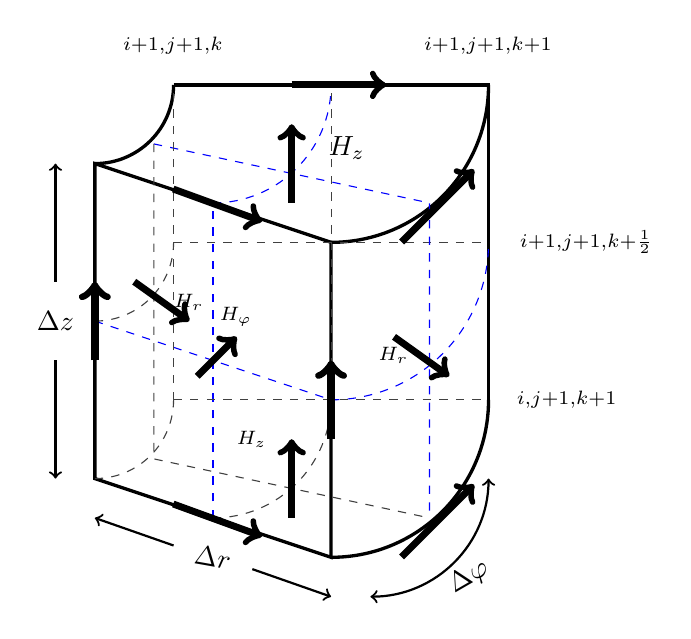
\begin{tikzpicture}
		%Разметка (потом убрать!)
		%\draw[help lines,ultra thin,step=.5cm](0,0) grid (8,8);
		%Основные прямые
		\draw [very thick] (1,1)--(1,5)--(4,4)--(4,0)--cycle;
		\draw [very thick] (2,6)--(6,6)--(6,2);
		
		%Основные Кривые %
		\draw [very thick] (1,5) to [out=0, in=270] (2,6); 
		\draw [very thick] (4,4) to [out=0, in=270] (6,6); 
		\draw [very thick] (4,0) to [out=0, in=270] (6,2); 
		
		%Кривые пунктиром %
		\draw [thin,dashed,color=blue] (4,2) to [out=0, in=270] (6,4); 
		\draw [thin,dashed,color=blue] (2.5,4.5) to [out=0, in=270] (4,6); 
		\draw [thin,dashed,color=darkgray] (1,3) to [out=0, in=270] (2,4);
		\draw [thin,dashed,color=darkgray] (2.5,0.5) to [out=0, in=270] (4,2); 
		\draw[thin,dashed,color=darkgray] (1,1) to [out=0, in=270] (2,2); 
		
		%Прямые Пунктиром		
		\draw[thin,dashed,color=blue] (1,3)--(4,2);
		\draw[thin,dashed,color=darkgray] (2,4)--(6,4);
		\draw[thin,dashed,color=blue] (2.5,0.5)--(2.5,4.5);
		\draw[thin,dashed,color=blue] (1.75,5.25)--(5.25,4.5)--(5.25,0.5);
		
		\draw[thin,dashed,color=darkgray] (1.75,5.25)--(1.75,1.25)--(5.25,0.5);
		\draw[thin,dashed,color=darkgray] (2,2)--(2,6);
		\draw[thin,dashed,color=darkgray] (2,2)--(6,2); 
		\draw[thin,dashed,color=darkgray] (4,2)--(4,6); 
		
		%Размеры сетки (дельты r, phi, z)
		%Дельта Z
		\draw[thick,<-] (0.5,1)--(0.5,2.5);
		\draw[thick,->] (0.5,3.5)--(0.5,5);
		\node at (0.5,3) {$\Delta z$};
		%Дельта r
		\draw[thick,<-] (1,0.5)--(2,0.15);
		\draw[thick,<-] (4,-0.5)--(3,-0.15);
		\node [rotate=-10]at (2.5,0) {$\Delta r$};
		%Дельта phi
		\draw[thick,<->] (4.5,-0.5) to [out=0,in=270] (6,1);
		\node [rotate=30]at (5.75,-0.25) {$\Delta \varphi$};
		%i,j,k
		\node[very thick] at (6,6.5){$_{i+1,j+1,k+1}$};
		\node[very thick] at (7.25,4){$_{i+1,j+1,k+\frac{1}{2}}$};
		\node[very thick] at (2,6.5){$_{i+1,j+1,k}$};
		\node[very thick] at (7,2){$_{i,j+1,k+1}$};
		%E
		\draw [line width=2.5,->,rotate around={-45:(5.25,0.5)}] (5.35,-0.1)--(5.35,1.2);
		\draw [line width=2.5,->,rotate around={-45:(5.25,4.5)}] (5.35,3.9)--(5.35,5.2);
		\draw [line width=2.5,->,rotate around={-110:(2.5,0.6)}] (2.60,0.1)--(2.60,1.3);
		\draw [line width=2.5,->,rotate around={-110:(2.5,4.6)}] (2.60,4.1)--(2.60,5.3);
		\draw [line width=2.5,->,rotate around={-90:(4,6.1)}] (4.1,5.6)--(4.1,6.8);
		\draw [line width=2.9,->] (1,2.5)--(1,3.5);
		\draw [line width=2.9,->] (4,1.5)--(4,2.5);
		%Hz
		\draw [line width=2.5,->] (3.5,4.5)--(3.5,5.5); \node[very thick] at (4.2,5.2){$H_{z}$};
		\draw [line width=2.5,->] (3.5,0.5)--(3.5,1.5); \node[very thick] at (3,1.5) {$_{H_{z}}$};
		%Hr
		\draw [line width=2.5,->] (4.8,2.8) node[very thick,below] {$_{H_{r}}$}--(5.5,2.3); 
		\draw [line width=2.5,->] (1.5,3.5)--(2.2,3)node[very thick,above] {$_{H_{r}}$};
		%Hphi
		\draw [line width=2.5,->] (2.3,2.3)--(2.8,2.8) node[very thick,above] {$_{H_{\varphi}}$}; 
	\end{tikzpicture}